\section{Results}

In this section we explore and discuss the results of our experiments with the machine learning, deep learning, and transformer models for Pashto poetry classification. We present the results of our experiments in the following subsections. 

The results can be summarized by the following table:

\begin{table}[ht]
    \centering
    \begin{tabular}{|l|c|}
        \hline
        \textbf{Model} & \textbf{Accuracy} \\
        \hline
        Logistic Regression & 62.88\% \\
        Support Vector Machine & 61.92\% \\
        Random Forest & 51.93\% \\
        XGBoost & 41.67\% \\
        \hline
    \end{tabular}
    \caption{Table of Results}
    \label{tab:results}
\end{table}

\subsection{Machine Learning Models}

This subsection presents the results of our experiments with the machine learning models. We used the following machine learning models for our experiments: Random Forest, Support Vector Machine, Logistic Regression, and XGBoost. The dataset was divided into 21844 samples for training, and 5465 samples for testing. The models were trained on an 8 Core, 4.90 GHz Intel Core i7-12700 CPU with 16GB RAM. 

\subsubsection{Random Forest}
Using 100 estimators, and a max depth of None, the Random Forest model achieved an accuracy of 51.93\%, and an F1 score of 0.50. The confusion matrix for the Random Forest model is shown below:
\begin{figure}[H]
    \centering
    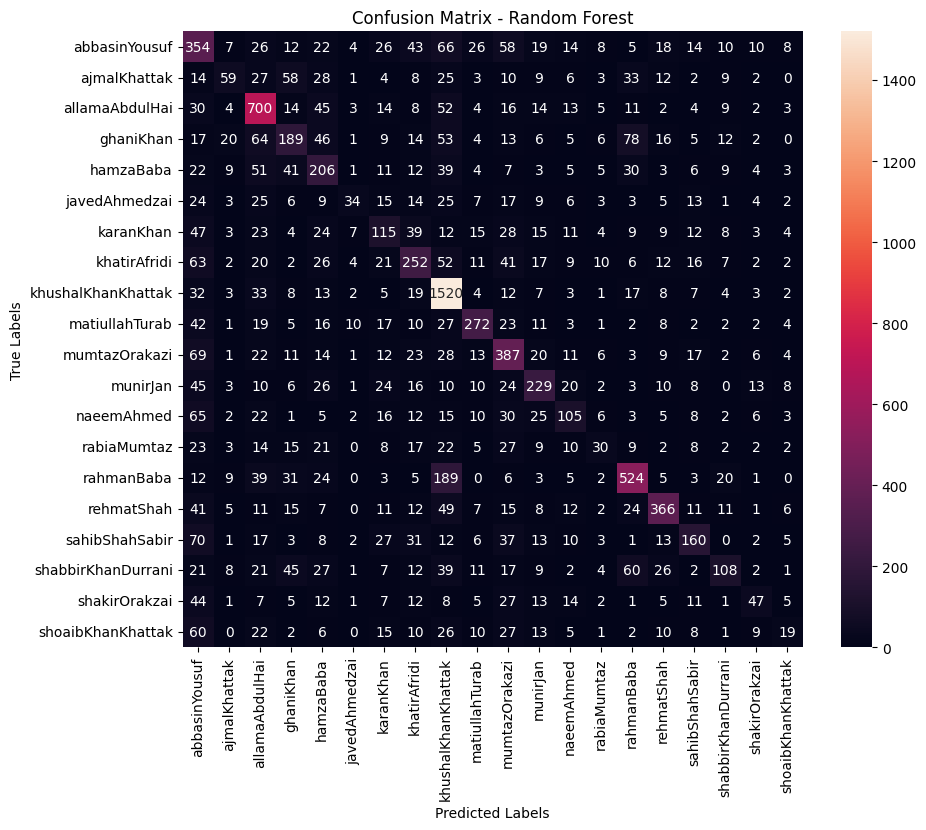
\includegraphics[width=0.45\textwidth]{rf_confmat.png}
\end{figure}

\subsubsection{Support Vector Machine}
With a C value of 1.0, an `rbf' kernel, and a gamma value of `scale', the Support Vector Machine model achieved an accuracy of 61.92\%, and an F1 score of 0.60. The confusion matrix for the Support Vector Machine model is shown below:
\begin{figure}[H]
    \centering
    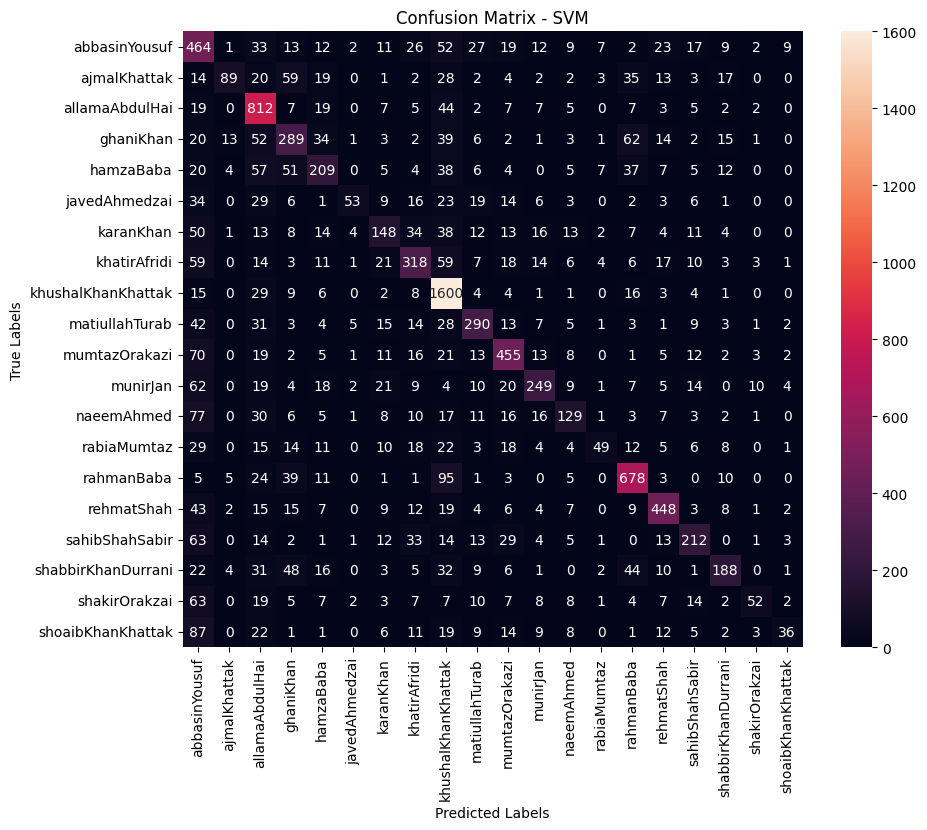
\includegraphics[width=0.45\textwidth]{svm_confmat.png}
\end{figure}

\subsubsection{Logistic Regression}
For the Logistic Regression model, our best hyperparameters turned out to be a C value of 10, max iterations of 1000, and a `newton-cg' solver. This gave an accuracy of 62.88\%, and an F1 score of 0.62. The confusion matrix for the Logistic Regression model is shown below:
\begin{figure}[H]
    \centering
    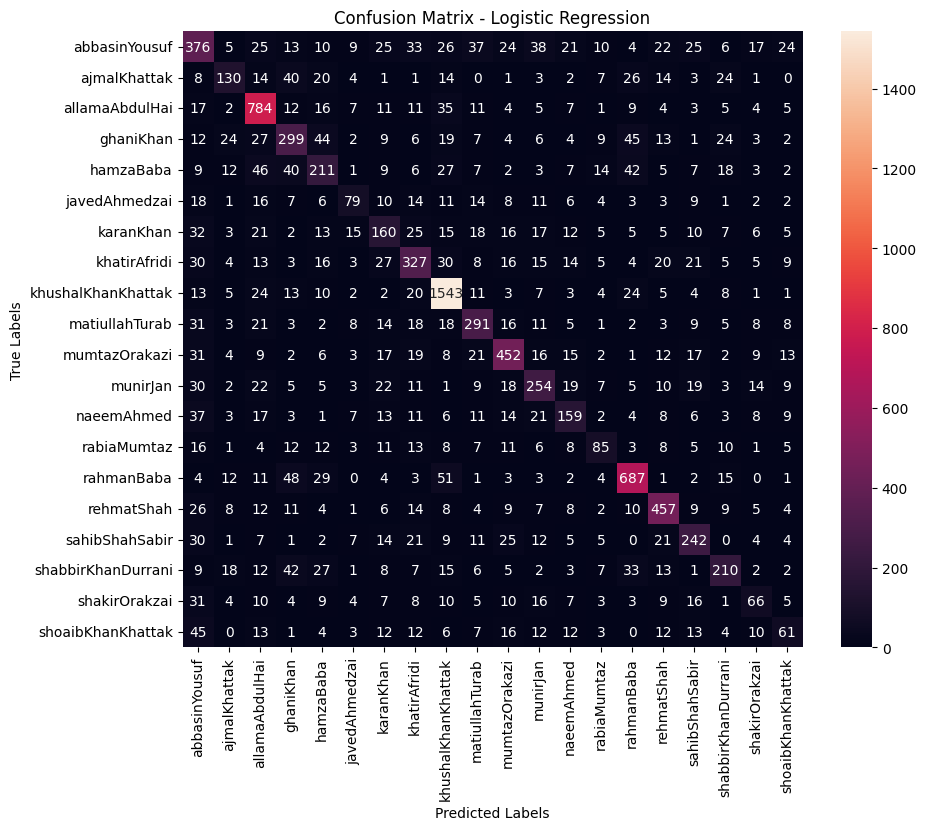
\includegraphics[width=0.45\textwidth]{logreg_confmat.png}
\end{figure}

\subsubsection{XGBoost}
Our best hyperparameters for XGBoost were 100 estimators, a learning rate of 0.1, max depth of 3, gamma value of 0.1, and a log-loss evaluation metric. This gave us an accuracy of 41.67\% and an F1 Score of 0.38. The confusion matrix for the XGBoost model is shown below:
\begin{figure}[H]
    \centering
    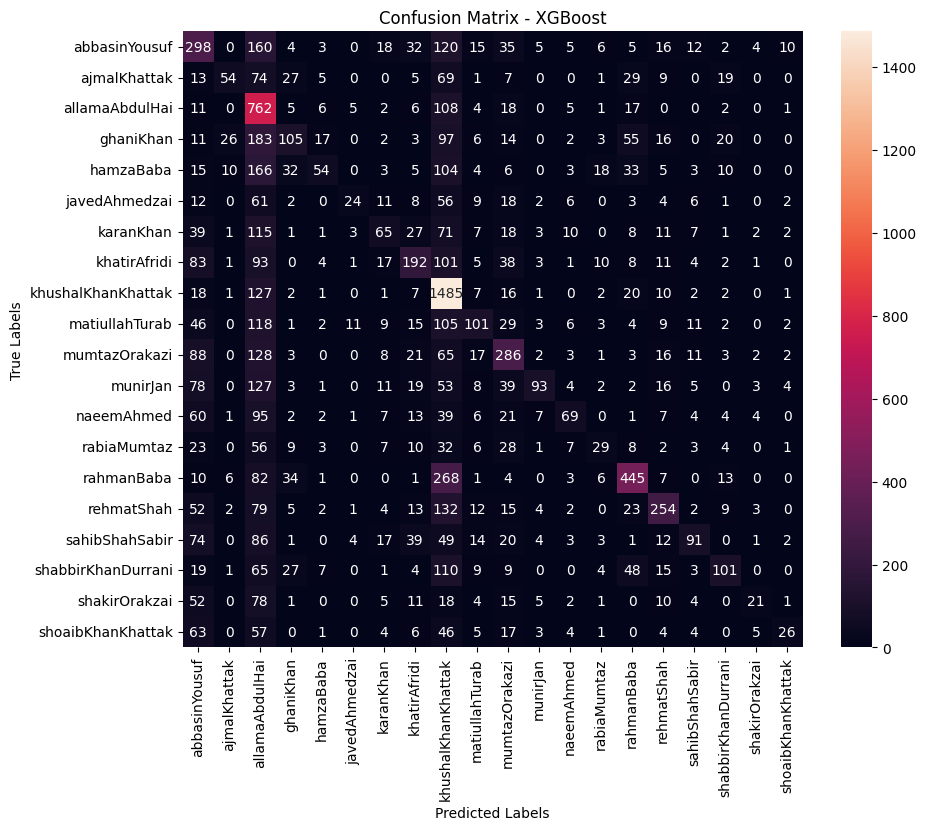
\includegraphics[width=0.45\textwidth]{xgboost_confmat.png}
\end{figure}

\subsection{Deep Learning Models}

This subsection presents the results of our experiments with the deep learning models. We used the following deep learning models for our experiments: LSTM and Bi-LSTM. The dataset was divided into 19111 samples for training, 2727 samples for validation, and 5471 samples for testing. They were trained on 2 Tesla T4 GPUs available on Kaggle, with Kaggle's 29GB RAM. 

\subsubsection{LSTM}
We experimented with various layers, and hyperparameters for LSTM including Bi-LSTM layers as well. The models were trained on 20 Epochs, with early stopping enabled. We experimented with a simple LSTM model with 2 LSTM layers of 128 and 64 units, respectively. We also added 2 dropout layers, and a dense layer with 64 units. The model was overfitting the training data, hence we continued with different parameters including compiling with an Adam Optimizer with a learning rate of 0.001, and a sparse categorical cross entropy loss, but that as well overfitted. 

\subsection{Transformer Models}

This subsection presents the results of our experiments with the transformer models. We used the following transformer models for our experiments: BERT, roBERTa, DistilBERT, and Meta Llama-3.2-1b. The embeddings were split into <> samples for training, <> samples for validation, and <> samples for testing. They were trained on 2 Tesla T4 GPUs available on Kaggle, with Kaggle's 29GB RAM.

\subsubsection{roBERTa}

\subsubsection{DistilBERT}

\subsubsection{Meta Llama-3.2-1b}


\subsection{Summary of Results}

This subsection presents a summary of the results of our experiments with the machine learning, deep learning, and transformer models for Pashto poetry classification.


